\chapter{코드로 그리는 기계: 파라메트릭 CAD}\label{ch:51-gear-cad}

\ref{ch:50-gear-mechanics}장의 치수는 문서(\code{layout.md}, 결정 0002)에 표로 적혀 있었다. 표의 숫자 하나하나는 계산으로
맞았다. 그런데 숫자가 맞는 것과 부품이 \emph{공간에서} 서로 비켜 들어가는 것은 다른 문제다. 이 장은 기어식 기계 전체를
Python 코드로 그리는 입체 모델(\code{hardware/gear/cad})을 다룬다. 마우스로 그리는 CAD 프로그램 없이, 스크립트가 부품
418개를 만들어 제자리에 놓고, 다른 스크립트가 그 모델을 재고 검사한다. 이 검사가 문서의 치수 아홉 개를 고치게 했고,
같은 모델의 숫자가 제어 보드의 시뮬레이션으로 그대로 흘러간다.

\section{왜 코드로 그리는가}\label{sec:gc-why}

\Why 기계 설계는 보통 마우스로 그리는 CAD 프로그램에서 한다. 스케치를 그리고 치수를 넣고 밀어 올려 입체를 만든다.
편하지만 이 프로젝트에는 맞지 않는 점이 셋 있다.

\begin{itemize}
\item \textbf{숫자의 출처.} 이 기계의 치수는 거의 모두 문서의 계산에서 나온다(축간 거리, 패드 면의 높이, 슬롯 각도).
CAD 파일 안에 숫자를 손으로 다시 넣으면 문서와 모델이 따로 놀기 시작한다. 숫자를 한 곳에 두고, 그 숫자가 어느 문서의
몇 절에서 왔는지를 옆에 적어 두고 싶다.
\item \textbf{검사.} ``부품끼리 겹치지 않는다'', ``덮개 틈이 4~mm 이하다'' 같은 조건을 사람이 눈으로 확인하면 고칠 때마다
다시 봐야 한다. 코드라면 검사도 코드로 쓰고, 고칠 때마다 돌리면 된다. \ref{ch:verify}장의 ``기준과 대조하는 자동
검사''를 기계에도 하는 것이다.
\item \textbf{변경의 기록.} 텍스트 파일은 저장소에서 무엇이 바뀌었는지 한 줄 단위로 보인다. CAD 프로그램의 이진 파일은
그렇지 않다.
\end{itemize}

치수를 이름 붙은 변수로 두고 모양을 그 변수의 함수로 만드는 방식을 \term{파라메트릭 설계}{parametric design}라 한다.
열 피치 120~mm를 바꾸면 열 모듈의 위치, 라인 축의 길이, 기계의 폭이 모두 따라 바뀐다.

\General 스프레드시트에서 합계 칸에 숫자를 직접 쳐 넣으면, 위의 칸 하나를 고쳤을 때 합계가 틀린 채 남는다. 합계 칸에
\code{=SUM(B2:B9)}라는 식을 넣으면 늘 맞는다. 파라메트릭 모델은 모든 부품의 모양과 자리가 이런 ``식''인 도면이다.
\ref{ch:boardgen}장에서 회로도와 기판을 Python으로 생성한 것도 같은 생각이었다.

\Ours 모델은 CadQuery 2.8로 만든다. CadQuery는 OpenCascade라는 공개 입체 모델링 엔진을 Python에서 부르는 라이브러리다.
파일의 역할은 그림~\ref{fig:gc-flow}와 같다.

\begin{figure}[ht]
\centering
\begin{tikzpicture}[x=1cm,y=1cm,
    f/.style={blk,font=\footnotesize\ttfamily,minimum width=24mm},
    o/.style={blkn,font=\footnotesize,minimum width=24mm},
    ar/.style={->,line width=0.7pt}]
  \node[blko,font=\footnotesize\ttfamily,minimum width=24mm] (p) at (0,0) {params.py};
  \node[note,anchor=south] at (0,0.5) {치수마다 출처\\(L, D, PCB, mod)};
  \node[f] (parts) at (3.2,0) {parts/*.py};
  \node[note,anchor=north] at (3.2,-0.5) {부품 하나 =\\함수 하나};
  \node[f] (b) at (6.2,0) {build.py};
  \node[note,anchor=north] at (6.2,-0.5) {부품 418개의 목록\\(이름, 모양, 역할)};
  \node[f] (c) at (9.4,1.4) {check.py};
  \node[f] (a) at (9.4,0) {assemble.py};
  \node[f] (r) at (9.4,-1.4) {render\_png.py};
  \node[o,anchor=west] (co) at (10.9,1.4) {80 PASS / 0 FAIL};
  \node[o,anchor=west] (ao) at (10.9,0) {STEP, SVG};
  \node[o,anchor=west] (ro) at (10.9,-1.4) {PNG};
  \draw[ar] (p) -- (parts); \draw[ar] (parts) -- (b);
  \draw[ar] (b) -- (c.west); \draw[ar] (b) -- (a.west); \draw[ar] (b) -- (r.west);
  \draw[ar] (c) -- (co); \draw[ar] (a) -- (ao); \draw[ar] (r) -- (ro);
  \node[blkg,font=\footnotesize\ttfamily,align=center] (fw) at (3.4,-2.7) {control-board/\\firmware\_model.py};
  \node[blkg,font=\footnotesize\ttfamily] (vc) at (7.6,-2.7) {verify\_control.py};
  \draw[ar,cgreen] (p) |- node[pos=0.75,above,font=\scriptsize,text=cgreen] {\code{SLOT\_STEPS}} (fw);
  \draw[ar,cgreen] (fw) -- (vc);
\end{tikzpicture}
\caption{CAD 파일의 흐름. 모든 숫자는 \code{params.py}에서 나온다. 검사(\code{check.py})도 기대값을 \code{params.py}와
문서에서 가져온다. 슬롯 원판의 각도는 기어식 제어 보드의 펌웨어 모델과 시뮬레이션이 같은 파일에서 읽는다(초록).}
\label{fig:gc-flow}
\end{figure}

모델의 결과물(기계 전체와 부분 조립의 STEP 파일)은 저장소 밖의 로컬 캐시 폴더에 둔다. 다시 만들 수 있는 산출물을
저장소에 넣지 않는 것은 보드 생성기와 같은 규칙이다. 보고서에 싣는 그림만 \code{report/figures/generated}에 쓴다.

\section{입체를 만드는 방법: 더하기와 빼기}\label{sec:gc-csg}

\Why 입체 모델링 엔진에서 가장 기본적인 연산은 세 가지 \term{불 연산}{Boolean operation}이다. 두 입체를 합치는 것
(합집합, \code{fuse}), 한 입체에서 다른 입체를 파내는 것(차집합, \code{cut}), 두 입체가 겹치는 부분만 남기는
것(교집합, \code{intersect}). 원기둥, 상자, 부채꼴 기둥 같은 단순한 입체를 이 세 연산으로 엮으면 웬만한 기계 부품이
된다. 이 방식을 \term{구성적 입체 기하}{constructive solid geometry, CSG}라 한다.

\General 목공에서 판재에 구멍을 뚫는 것은 판(상자)에서 드릴 날의 궤적(원기둥)을 빼는 것이다. 쿠키 틀로 반죽을 찍어
내는 것은 반죽과 틀의 교집합이다.

\Ours 모델의 모든 부품이 이렇게 만들어진다. 공용 도우미 \code{parts/\_util.py}에는 두 점 사이의 원기둥(\code{cyl}),
속이 빈 원기둥(\code{tube}), 부채꼴 기둥(\code{sector}) 같은 단순 입체가 있다. 자리올림의 잠금 원판(\ref{sec:gm-carry}절)은
둥근 원판에서 가장자리의 작은 원기둥 26개를 빼서 만든다(그림~\ref{fig:gc-csg}).

\begin{lstlisting}[language=Python,caption={\code{parts/gearing.py}: 잠금 원판 = 원판 $-$ 원기둥 26개.},label={lst:gc-lock}]
def lock_disc(r_l, pocket_half, width):
    """Driven-side lock disc: radius R_L, 26 concave pockets (circular notches of half width pocket_half)."""
    s = tubez(r_l, BORE, 0.0, width)
    cuts = []
    for k in range(P.N_CH):
        x, y = polar(r_l, 360.0 / P.N_CH * k + 90.0)
        cuts.append(cylz(pocket_half, -1, width + 1, x, y))
    return s.cut(*cuts)
\end{lstlisting}

빼는 원기둥을 원판보다 위아래로 1~mm씩 길게(\code{-1}부터 \code{width + 1}까지) 만드는 데 주목하자. 빼는 입체와 빼이는
입체의 면이 정확히 같은 높이에 있으면, 엔진의 계산 오차 때문에 두께 0의 얇은 막이 남거나 연산이 실패하기 쉽다. 조금
넘치게 자르는 것은 CSG의 오래된 요령이다.

\begin{figure}[ht]
\centering
\begin{tikzpicture}[x=1cm,y=1cm]
  \def\s{0.045}
  \begin{scope}
    \fill[cgreenbg,draw=cgreen] (0,0) circle (27*\s); \fill[white,draw=cgreen] (0,0) circle (10*\s);
    \node[note,anchor=north] at (0,-1.45) {\code{tubez(27, 10, ...)}};
  \end{scope}
  \node[font=\Large] at (1.9,0) {$-$};
  \begin{scope}[xshift=3.8cm]
    \foreach \i in {0,...,25} \draw[corange] ({90+\i*360/26}:{27*\s}) circle (2.8*\s);
    \draw[cgray,dashed] (0,0) circle (27*\s);
    \node[note,anchor=north] at (0,-1.45) {\code{cylz(2.8, ...)} × 26};
  \end{scope}
  \node[font=\Large] at (5.7,0) {$=$};
  \begin{scope}[xshift=7.6cm]
    \fill[cgreenbg] (0,0) circle (27*\s);
    \foreach \i in {0,...,25} \fill[white] ({90+\i*360/26}:{27*\s}) circle (2.8*\s);
    \draw[cgreen] (0,0) circle (27*\s);
    \fill[white,draw=cgreen] (0,0) circle (10*\s);
    \node[note,anchor=north] at (0,-1.45) {잠금 원판 (오목한 자리 26개)};
  \end{scope}
\end{tikzpicture}
\caption{차집합으로 만든 잠금 원판(자리올림 1, 반지름 27~mm, 자리의 반폭 2.8~mm).}
\label{fig:gc-csg}
\end{figure}

\section{\texorpdfstring{\code{params.py}}{params.py}: 숫자는 한 곳에만}\label{sec:gc-params}

\Why 모델 전체에서 숫자가 사는 곳은 \code{params.py} 하나다. 다른 파일에는 숫자를 쓰지 않고 이 파일의 이름만 부른다.
그리고 숫자마다 출처를 적는다. 머리말이 규칙을 밝힌다.

\begin{lstlisting}[language=Python,caption={\code{params.py}의 머리말: 출처 표기의 규칙.},label={lst:gc-head}]
Units: mm and degrees.  Every value cites its origin:
  L<x.y>  = hardware/gear/layout.md section x.y
  D<n>    = docs/decisions/0002-gear-detail-decisions.md section n
  PCB     = hardware/gear/drum-pcb/README.md
  D1      = docs/decisions/0001-test-register-timing.md (via layout 3.8)
  (mod)   = a modelling choice made in this CAD (not a design value); see README.md
\end{lstlisting}

\code{(mod)}가 중요하다. 문서에는 없지만 입체를 그리려면 정해야 하는 값이 있다. 판 사이 기둥의 지름, 센서 브래킷의 바깥
치수 같은 것이다. 이런 값에 \code{(mod)}를 달아 두면, 나중에 읽는 사람이 ``이 숫자는 설계 결정이 아니라 그림을 위한
가정''임을 안다. 설계 값과 모델링의 편의를 섞지 않는 것이다.

\Ours 몇 줄을 보자.

\begin{lstlisting}[language=Python,caption={\code{params.py}에서 발췌.},label={lst:gc-params}]
PITCH = 120.0                     # L3.6, D13: column pitch (also row pitch)
FRAME_END = 40.0                  # L3.9: 40 + 12*120 + 360 + 40
DRIVE_W = 360.0                   # D4: drive module width
BANK_W = FRAME_END + N_SLOTS * PITCH + DRIVE_W + FRAME_END     # = 1880  (L3.9, D13)
...
Z_PAD = 27.0                      # pad plane
BOARD_Z0, BOARD_Z1 = 16.4, 18.0   # D3: contact board +18.0 ... +16.4
...
C_FI, C_IC, C_CM, C_MS = 39.0, 42.0, 39.0, 120.0   # L3.7 spec centre distances
...
LOCK_R1, LOCK_R2 = 27.0, 43.0     # D8: lock disc radius R_L (carry 1 / 2)
LOCK_GAP = 0.05                   # D8: radial gap 0.05
...
MOTOR_CENTRE_DIST = 103.6         # D5: C = 103.6
MOTOR_AXIS_DY = math.sqrt(MOTOR_CENTRE_DIST ** 2 - MOTOR_AXIS_DZ ** 2)   # 76.4 (L3.7: about 76)
\end{lstlisting}

다른 값에서 \emph{계산되는} 값은 계산식으로 적는다. 기계의 폭 1,880~mm는 직접 쓰지 않고 끝판 + 12 × 열 피치 + 구동부 +
끝판으로 쓴다. 모터 축의 높이는 벨트의 축간 거리 103.6~mm와 뒤로 물린 거리 70~mm에서 피타고라스의 정리로 나온다.
문서에는 ``약 76''이라고 적혀 있고, 모델은 76.4를 쓴다. 이렇게 하면 열 피치를 바꿨을 때 폭이 저절로 바뀌고, 문서의
반올림한 값과 모델의 정확한 값이 어디서 갈렸는지가 주석에 남는다.

\section{부품은 함수, 기계는 부품의 목록}\label{sec:gc-parts}

\Why 부품 하나를 만드는 일은 함수 하나로 적는다. 함수는 원점에 놓인 입체를 돌려주고, 그것을 기계 안의 어디에 놓을지는
따로 정한다. 같은 드럼을 18자리에 놓아야 하므로 모양과 자리를 나누는 것이 자연스럽다.

\paragraph{V홈을 파는 칼.} 인덱스 플랜지의 V홈(\ref{sec:gm-brake}절)은 깊이가 반지름에 비례한다($\pi r / 26$). 반지름마다
단면이 다른 홈이다. 이것을 파내는 칼은 \term{로프트}{loft}로 만든다. 로프트는 서로 다른 두 단면을 직선으로 이어 입체를
만드는 연산이다. 안쪽 반지름의 작은 V자 삼각형과 바깥쪽 반지름의 큰 V자 삼각형을 이으면, 반지름을 따라 일정한 비율로
커지는 쐐기가 된다(그림~\ref{fig:gc-loft}). 이 쐐기를 13.846°씩 돌려 가며 26번 빼면 플랜지가 된다.

\begin{lstlisting}[language=Python,caption={\code{parts/index.py}: 반지름에 비례해 깊어지는 V홈의 칼과 플랜지.},label={lst:gc-groove}]
def _groove_cutter():
    r1, r2 = P.GROOVE_R_CUT
    m = 0.6

    def tri(r):
        d = P.groove_depth(r)
        return [(-(d + m), m + P.FLANGE_Z1), (d + m, m + P.FLANGE_Z1), (0.0, -d + P.FLANGE_Z1)]
    wp = (cq.Workplane("YZ", origin=(r1, 0, 0)).polyline(tri(r1)).close()
          .workplane(offset=r2 - r1).polyline(tri(r2)).close().loft(ruled=True))
    return wp.val()

def index_flange():
    """O34 x 5.6 flange (Z 18 ... 23.6), O8 bore, 26 radial 90-deg V grooves, depth pi*r/26."""
    s = cylz(P.FLANGE_D / 2, P.FLANGE_Z0, P.FLANGE_Z1)
    s = s.cut(cylz(P.SHAFT_D / 2, P.FLANGE_Z0 - 1, P.FLANGE_Z1 + 1))
    cutter = _groove_cutter()
    cutters = [rotz(cutter, pad_angle(k)) for k in range(P.N_CH)]
    return s.cut(*cutters)
\end{lstlisting}

삼각형 \code{tri(r)}의 두 위 꼭짓점은 $(\pm(d+m),\ \text{면} + m)$, 아래 꼭짓점은 $(0,\ \text{면} - d)$다. 옆으로 $d$, 아래로
$d$이므로 경사면이 45°, 곧 홈의 각이 90°다. 위로 \code{m} = 0.6~mm 넘치게 그린 것은 앞 절의 ``조금 넘치게 자른다''와
같은 이유다.

\begin{figure}[ht]
\centering
\begin{tikzpicture}[x=1cm,y=1cm]
  % radial axis to the right, triangles drawn in perspective
  \draw[->,cgray] (-0.4,0) -- (6.4,0) node[right,font=\scriptsize] {반지름 $r$};
  \coordinate (a1) at (0.6,0.0); \coordinate (a2) at (1.6,0.0);
  % small triangle at r1 (depth 1.0 units), large at r2 (depth 1.7 units) drawn in a pseudo-3D view
  \filldraw[corange!60,draw=corange] (0.2,1.0) -- (1.4,1.0) -- (0.8,0.4) -- cycle;
  \filldraw[corange!35,draw=corange] (4.1,1.3) -- (6.1,1.3) -- (5.1,0.0) -- cycle;
  \draw[corange,dashed] (0.2,1.0) -- (4.1,1.3); \draw[corange,dashed] (1.4,1.0) -- (6.1,1.3); \draw[corange,dashed] (0.8,0.4) -- (5.1,0.0);
  \node[note,anchor=north] at (0.8,0.25) {$r_1 = 10.5$:\\깊이 $\pi r_1/26$};
  \node[note,anchor=north] at (5.1,-0.15) {$r_2 = 17.5$:\\깊이 $\pi r_2/26$};
  \node[note,text=corange] at (3.0,1.65) {두 단면을 직선으로 이음(로프트)};
  % flange top view with cutters
  \begin{scope}[xshift=9.6cm,yshift=0.5cm]
    \def\s{0.075}
    \fill[cgray!25,draw=cgray] (0,0) circle (17*\s); \fill[white,draw=cgray] (0,0) circle (4*\s);
    \foreach \i in {0,...,25} {
      \pgfmathsetmacro{\a}{90-\i*360/26}
      \fill[corange!60,rotate=\a] ({10.5*\s},{-0.9*\s}) -- ({17.5*\s},{-1.6*\s}) -- ({17.5*\s},{1.6*\s}) -- ({10.5*\s},{0.9*\s}) -- cycle;
    }
    \node[note,anchor=north] at (0,-1.45) {칼 26개를 돌려 놓고 한 번에 뺀다};
  \end{scope}
\end{tikzpicture}
\caption{V홈을 파는 칼. 왼쪽: 안쪽과 바깥쪽 반지름의 V자 단면을 이은 쐐기(로프트). 오른쪽: 플랜지(지름 34~mm) 위에
26개를 돌려 놓은 모습(위에서 본 칼의 자취).}
\label{fig:gc-loft}
\end{figure}

\paragraph{설계의 식이 그대로 코드가 된다.} 자리올림의 잠금 원호 반지름은 ``축간 거리 $-$ 잠금 원판의 반지름 $-$
틈''이다(결정 0002의 8절). 코드도 그 문장 그대로다.

\begin{lstlisting}[language=Python,caption={\code{parts/gearing.py}: 잠금 원호의 반지름과 자리올림 1.},label={lst:gc-carry}]
def lock_arc_radius(centre_dist, lock_r):
    """Radius of the convex locking arc on the driver: centre distance - lock disc radius - gap (D8)."""
    return centre_dist - lock_r - P.LOCK_GAP

def carry1():
    ...
    r_arc = lock_arc_radius(P.C_CM, P.LOCK_R1)
    tip = P.CARRY1_DRV_PD / 2 + P.CARRY1_M          # tooth tip radius of the 13T equivalent
    return {
        "drv_tooth": tooth_disc(r_arc, tip, 360.0 / (2 * P.CARRY1_TOOTH_EQ_T), P.GEAR_W),
        "drv_arc": arc_disc(r_arc, P.LOCK_W),
        "drn_gear": gear_env(P.CARRY1_M * P.CARRY1_DRIVEN_T / 2, P.GEAR_W),
        "drn_lock": lock_disc(P.LOCK_R1, P.LOCK_POCKET_HALF[0], P.LOCK_W),
        ...
\end{lstlisting}

자리올림 1이면 $39 - 27 - 0.05 = 11.95$~mm다. 자리올림 2는 같은 함수에 축간 거리 120과 잠금 원판 43을 넣어 76.95~mm가
나온다. 이 값이 다음 절에서 문서의 ``약 78''과 어긋난다.

\paragraph{무엇을 단순하게 그렸는가.} 기어는 이를 하나하나 그리지 않고 \emph{피치원 크기의 원기둥}으로 그린다. 마이터
기어는 피치 원뿔의 겉껍질이다. 맞물리는 두 기어의 원기둥은 정확히 맞닿아 겹치는 부피가 0이다. 이 모델의 목적은 이의
접촉을 해석하는 것이 아니라 축의 자리, 부품 사이의 틈, 외형을 확인하는 것이기 때문이다. 나사, 리본 케이블, 접시
스프링, 인쇄는 그리지 않는다. 무엇을 생략했는지는 \code{cad/README.md}에 목록으로 있다. 단순화를 \emph{적어 두는}
것이 중요하다. 그래야 ``모델에서 간섭이 0''이 무엇에 대해 0인지 안다.

\paragraph{조립: 이름 붙은 부품의 목록.} \code{build.py}의 \code{Model}은 부품의 평평한 목록이다. 부품마다 이름, 모양,
묶음(STEP 파일을 나눌 단위), \emph{역할}(\code{moving} 또는 \code{static}), 색을 갖는다. 열 모듈 하나를 놓는 함수는
행마다 같은 부품들을 그 높이에 놓는다.

\begin{lstlisting}[language=Python,caption={\code{build.py}: 열 모듈 하나(발췌).},label={lst:gc-column}]
def build_column(m, slot, grp=None):
    g = grp or f"column_{slot:02d}"
    x = P.slot_x(slot)
    ...
    for row in P.ROW_ORDER:
        y = P.ROW_Y[row]
        n = f"{s}_{row}"
        ...
        m.add(f"{n}_shaft", at(shaft.drum_shaft(), x, y), g, "moving", "steel")
        ...
        m.add(f"{n}_flange", at(index.index_flange(), x, y), g, "moving", "steel")
        ...
        m.add(f"{n}_board", at(board.contact_board(), x, y), g, "static", "pcb")
        m.add(f"{n}_contacts", at(board.contact_pins(), x, y), g, "static", "gold")
        ...
        m.add(f"{n}_drum_pads", at(drum.drum_pads(), x, y), g, "moving", "gold")
        ...
\end{lstlisting}

역할을 붙이는 이유는 다음 절의 간섭 검사가 ``움직이는 것과 서 있는 것이 부딪히는가''를 따로 세기 때문이다. 같은
함수(\code{index\_flange})를 열여덟 번 부르지만, 함수에 \code{@lru\_cache}를 달아 모양은 한 번만 계산하고 옮기기만 한다.
기계 전체를 만드는 데 약 6초가 걸린다.

라인 축의 마이터 기어를 놓는 줄에 \ref{sec:gm-train}절의 회전 방향이 한 글자로 들어 있다.
\begin{lstlisting}[language=Python,numbers=none]
            sign = -1 if row == "mid" else 1               # D7: middle row on the opposite side
\end{lstlisting}

\section{\texorpdfstring{\code{check.py}}{check.py}: 모델이 스스로를 잰다}\label{sec:gc-check}

\Why 모델을 만들었으면 문서의 숫자와 맞는지 재야 한다. \code{check.py}는 모델을 만든 뒤 부품의 경계 상자와 부피를 읽어
약 80가지를 잰다. 결과는 표 한 장이고, 하나라도 \code{FAIL}이면 종료 코드 1로 끝난다.

\begin{itemize}
\item \textbf{구동부}: 축간 거리 F--I 39, I--C 42, C--M 39와 그 합 120, M--S 120, 다섯 축이 한 평면($Z = -109$)에 있는가.
맞물리는 두 기어의 피치 반지름의 합이 축간 거리와 같은가. 벨트 길이가 450~mm인가. 슬롯 원판 세 트랙의 각도와
타이밍 여유(\ref{sec:gc-slotsteps}절). 브레이크가 자리올림 2의 이 끝과 2~mm 이상 떨어져 있는가.
\item \textbf{드럼 자리}: 패드 면이 $Z = +27.000$인가. 접점 공의 꼭대기가 패드 면과 같은가(눌린 상태 9.0~mm). 접점 104개,
패드 104개. 인덱스 핀이 봉우리 면보다 0.7 / 1.4~mm 아래인가. 플랜지에서 파낸 V홈의 부피가 해석적으로 계산한 값과
6\% 안에서 같은가.
\item \textbf{배치와 외형}: 드럼 사이 피치 120, 이웃 드럼 몸체 사이 20~mm, 외형 1,880 × 1,350 × 403~mm(허용 $\pm5$).
\item \textbf{덮개}: 앞 덮개와 고정 테 사이의 틈이 4~mm 이하, 앞 덮개에서 가장 가까운 움직이는 부품(노브)까지 20~mm
이상(결정 0002의 10절, 손가락이 닿지 않을 거리).
\end{itemize}

V홈의 부피 검사는 ``모양이 맞는가''를 숫자 하나로 확인하는 요령이다. 홈의 단면은 깊이 $d = \pi r/26$인 직각 이등변
삼각형이고 넓이는 $d^2$이다. 이것을 반지름을 따라 적분하면 홈 26개의 부피가 $26 (\pi/26)^2 (r_2^3 - r_1^3)/3$으로 나온다.
모델에서 파낸 부피(원래 원판의 부피 $-$ 플랜지의 부피)가 이 값과 맞으면 칼의 모양과 개수와 깊이가 맞는 것이다.

\subsection{간섭 검사: 겹치는 부피를 잰다}

\Why 부품 두 개가 부딪히는지는 두 입체의 교집합 부피로 안다. 부피가 0이면 비켜 있거나 맞닿아 있고, 0보다 크면 서로를
파고든다. 문제는 쌍의 수다. 부품이 418개이면 쌍은 $418 \times 417 / 2 = 87{,}153$개이고, 불 연산 하나는 수십 밀리초가
걸린다.

\General 컴퓨터 게임의 충돌 판정이 같은 문제를 두 단계로 푼다. 먼저 물체마다 그것을 감싸는 상자(\term{경계 상자}{bounding
box})를 두고, 상자끼리 겹치는 쌍만 고른다(\term{넓은 단계}{broad phase}). 상자 비교는 부등식 여섯 개라 매우 빠르다.
그렇게 남은 소수의 쌍에 대해서만 실제 모양으로 정밀하게 판정한다(\term{좁은 단계}{narrow phase}). 상자가 겹치지 않으면
속의 물체도 겹칠 수 없으므로 첫 단계에서 버린 쌍은 확실히 안전하다(그림~\ref{fig:gc-bbox}).

\begin{figure}[ht]
\centering
\begin{tikzpicture}[x=1cm,y=1cm]
  \foreach \dx/\ttl/\case in {0/{상자가 떨어짐: 버림}/0,4.6/{상자는 겹침, 모양은 비킴}/1,9.2/{모양이 겹침: 부피 $> 0$}/2} {
    \begin{scope}[xshift=\dx cm]
      \node[font=\footnotesize\bfseries] at (1.6,2.3) {\ttl};
      \fill[cbluebg,draw=cblue] (0.5,1.0) circle (0.6);
      \draw[cblue,dashed] (-0.1,0.4) rectangle (1.1,1.6);
      \ifcase\case
        \fill[corangebg,draw=corange] (2.6,0.8) -- (3.4,0.8) -- (3.4,1.8) -- cycle;
        \draw[corange,dashed] (2.6,0.8) rectangle (3.4,1.8);
      \or
        \fill[corangebg,draw=corange] (0.95,0.3) -- (2.2,0.3) -- (2.2,1.5) -- cycle;
        \draw[corange,dashed] (0.95,0.3) rectangle (2.2,1.5);
      \or
        \fill[corangebg,draw=corange,fill opacity=0.8] (0.7,0.5) rectangle (1.9,1.4);
        \draw[corange,dashed] (0.7,0.5) rectangle (1.9,1.4);
        \begin{scope}
          \clip (0.5,1.0) circle (0.6);
          \fill[cred] (0.7,0.5) rectangle (1.9,1.4);
        \end{scope}
      \fi
    \end{scope}}
  \node[note,anchor=north] at (6.2,0.05) {점선 = 경계 상자. 상자가 겹치는 쌍만 불 연산으로 부피를 잰다.};
\end{tikzpicture}
\caption{넓은 단계와 좁은 단계. 빨간 부분이 교집합이다.}
\label{fig:gc-bbox}
\end{figure}

\Ours \code{check.py}는 넓은 단계를 numpy의 배열 비교로 한꺼번에 한다.

\begin{lstlisting}[language=Python,caption={\code{check.py}: 경계 상자로 쌍을 고른 뒤 교집합 부피를 잰다(발췌).},label={lst:gc-interf}]
    arr = np.array([[b.xmin, b.xmax, b.ymin, b.ymax, b.zmin, b.zmax] for b in boxes])
    pairs = []
    for i in range(n):
        ov = ((np.minimum(arr[i, 1], arr[i + 1:, 1]) - np.maximum(arr[i, 0], arr[i + 1:, 0]) > BBOX_EPS) &
              (np.minimum(arr[i, 3], arr[i + 1:, 3]) - np.maximum(arr[i, 2], arr[i + 1:, 2]) > BBOX_EPS) &
              (np.minimum(arr[i, 5], arr[i + 1:, 5]) - np.maximum(arr[i, 4], arr[i + 1:, 4]) > BBOX_EPS))
        for j in np.nonzero(ov)[0]:
            pairs.append((i, i + 1 + int(j)))
    ...
    for i, j in todo:
        a, b = parts[i], parts[j]
        v = a.shape.intersect(b.shape).Volume()
        ...
        if v > VOL_TOL:
            bad.append((a.name, b.name, v))
\end{lstlisting}

두 구간 $[a_0, a_1]$과 $[b_0, b_1]$이 겹치는 길이는 $\min(a_1, b_1) - \max(a_0, b_0)$이다. 이것이 세 축 모두에서 양수이면
상자가 겹친다. 87,153쌍 가운데 683쌍만 남고, 그중 18쌍(패드가 기판 면에 묻히도록 일부러 그린 금 도금과 기판의 짝)을
빼면 665쌍을 불 연산으로 잰다. 약 20초다.

판정의 문턱 \code{VOL\_TOL}은 0.5~mm$^3$이다. 맞닿아야 하는 면(인덱스 핀과 V홈의 경사면, 맞물린 기어의 원기둥)에서는
엔진이 0 대신 아주 작은 부피를 내기 때문이다. 지금 모델에서 가장 큰 것은 0.033~mm$^3$이다. 결과는 세 갈래로 나누어 센다.
움직이는 부품 대 서 있는 부품, 움직이는 부품끼리, 서 있는 부품끼리. 모두 0이어야 한다.

\paragraph{검사기를 검사한다.} ``간섭 0''은 검사가 아무것도 보지 않아도 나온다. 그래서 \code{check.py}는 끝에 일부러
틀린 모델을 만들어 검사기가 잡는지 본다(\ref{sec:v-mutants}절의 음성 시험과 같은 생각이다).

\begin{lstlisting}[language=Python,caption={\code{check.py}: 자기 시험. 드럼을 접점 쪽으로 1~mm 밀어 넣는다.},label={lst:gc-self}]
def selftest(tab):
    m = build.Model()
    build.build_column(m, 12)
    for p in m.parts:
        if p.name.startswith("s12_mid_drum_") or p.name == "s12_mid_index_disc":
            p.shape = p.shape.translate(cq.Vector(0, 0, -1.0))
    t = Table()
    interference(m, t)
    hits = [r for r in t.rows if r[0].startswith(("moving parts vs", "static vs")) and r[3] == "FAIL"]
    tab.add("self-test: drum shifted 1 mm onto the contacts is detected", ">= 1 failing class", ...)
\end{lstlisting}

드럼을 1~mm 밀면 접점의 공이 기판을 파고든다. 이것이 \code{FAIL}로 잡히지 않으면 자기 시험이 실패하고 전체가 실패한다.
실제로도 이 검사가 일을 했다. F 축 브레이크(\ref{sec:gm-brake}절)를 처음 놓은 자리(구동부 좌표 $u$ = 61--97~mm)가 아이들
축 I의 끝과 105~mm$^3$ 겹친다는 것을 간섭 검사가 잡았고, 자리를 59--92~mm로 옮겼다.

\paragraph{FAIL과 OPEN.} 검사에는 세 가지 결과가 있다. \code{PASS}, \code{FAIL}, 그리고 \code{OPEN}이다. \code{OPEN}은
``문서에 적힌 값으로는 기하학적으로 닫히지 않아 모델에서는 다른 값을 쓴 항목''이다. 종료 코드에는 영향을 주지 않지만
표에 늘 남아서 사람이 결정해야 할 것임을 보인다. 마지막 실행 결과는 80 PASS, 0 FAIL, 6 OPEN이다.

\section{모델이 찾아낸 것}\label{sec:gc-found}

모델을 처음 만들었을 때 문서의 치수 아홉 개가 공간에서 닫히지 않았다(표~\ref{tab:gc-found}). 결정 0002와 \code{layout.md}는
``CAD 반영'' 절을 두어 모델의 값으로 고쳤고, 확정하지 못한 것은 열린 항목으로 남겼다.

\begin{table}[ht]
\centering
\caption{상세 CAD에서 바뀐 치수(결정 0002 ``CAD 반영''). 문서의 계산은 각각 맞았지만 다른 부품과 만나는 곳에서 어긋났다.}
\label{tab:gc-found}
\small
\begin{tabularx}{\linewidth}{>{\raggedright\arraybackslash}p{8mm}>{\raggedright\arraybackslash}p{30mm}>{\raggedright\arraybackslash}p{30mm}>{\raggedright\arraybackslash}X}
\toprule
& 항목 & 문서 $\to$ 모델 & 왜 닫히지 않았나 \\
\midrule
C1 & 위치 원판 & 지름 60 $\to$ 56 & F와 M의 원판 옆 39~mm에 축 I, C(지름 20)가 지난다. 반지름은 $39 - 10 = 29$ 이하여야 한다 \\
C2 & 구동부 옆판의 베어링 & 6004 $\to$ 6804 & 축간 39~mm에 바깥지름 42~mm 베어링 두 개는 들어가지 않는다(3~mm 겹침) \\
C3 & 인덱스 홈의 띠 & $r$ 11--16.5 $\to$ 10.5--17.5 & 길이 6~mm의 핀이 6.9° 기울어 반지름 방향으로 $6 \cos 6.9° = 5.96$~mm를 차지한다. 띠는 5.5~mm \\
C4 & 자리올림 2의 잠금 원호 & 약 78 $\to$ 76.95 & 78은 \emph{이빨} 평면의 한계였다. \emph{잠금} 평면에서는 $R_a + R_L + 0.05 = 120$ \\
C5 & 기준 바 & 세움 $\to$ 눕힘 & 뱅크 바닥과 열 모듈 판 사이가 30~mm뿐이라 50~mm 높이로 세울 수 없다 \\
C6 & 옆·위 덮개 & 프로파일 밖 $\to$ 3~mm 매립 & 밖에 붙이면 폭이 1,886~mm로 허용($\pm5$)을 벗어난다 \\
C7 & 지시 드럼의 뒤판 & 116 $\to$ 70 & 116~mm 판은 구동부 옆판 A를 가로지른다 \\
C8 & 마이터의 길이 & 약 29 $\to$ 23.5 & 피치 원뿔로 그린 길이. 카탈로그 확인 전 \\
C9 & 모터 공간 & 위 약 10 $\to$ 7.6 & 모터에 맞춰 뒤 레일, 기둥, 옆판을 고친 뒤의 실제 틈 \\
\bottomrule
\end{tabularx}
\end{table}

\begin{lesson}{숫자는 맞았는데 부품이 들어가지 않았다}
C1이 전형이다. \code{layout.md}는 위치 원판을 지름 60~mm로 적었다. 원판에 슬롯 26개를 내기에 알맞은 크기였고, 그 자체로는
문제가 없었다. 다른 절은 F와 I의 축간 거리를 39~mm로, 라인 축의 지름을 20~mm로 적었다. 이것도 맞다. 그런데 F의 원판
바로 옆을 I 축이 지나간다는 사실은 어느 표에도 함께 적혀 있지 않았다. 두 숫자가 \emph{만나는 곳}은 공간이고, 공간에서
둘을 함께 놓아 보는 것은 모델이 처음이었다. 간섭 검사가 겹침을 내고, \code{OPEN} 항목이 문서의 값과 모델의 값을 나란히
보였다. C4도 비슷하다. ``약 78''은 이빨이 지나가는 평면에서 잰 한계였는데, 잠금 원호는 그 옆의 다른 평면에 있고 거기서는
축간 거리 120에서 잠금 원판의 반지름 43과 틈을 뺀 76.95가 맞다. 문서를 쓰는 사람은 한 번에 한 부품을 본다. 모델은 모든
부품을 한꺼번에 본다.
\end{lesson}

\section{\texorpdfstring{\code{SLOT\_STEPS}}{SLOT\_STEPS}: 기계와 제어 보드가 같은 숫자를 읽는다}\label{sec:gc-slotsteps}

\Why 슬롯 원판의 각도는 두 곳에서 쓰인다. CAD는 원판에 슬롯을 판다. 제어 보드의 펌웨어 모델과 시뮬레이션은 슬롯이
센서를 지나는 순간을 계산해 \code{STROBE}, \code{JUDGE}, \code{CLEAR}의 시각을 얻는다(\ref{ch:52-gear-control}장).
두 곳에 같은 숫자를 따로 적어 두면 언젠가 하나만 고쳐진다. 그러면 시뮬레이션은 통과하는데 실제 원판은 다른 각도로
깎인다. 그래서 숫자는 \code{params.py} 한 곳에 두고 제어 보드 쪽이 그 파일을 읽는다.

\Ours 각도는 도가 아니라 \emph{모터 스텝}으로 적는다.

\begin{lstlisting}[language=Python,caption={\code{params.py}: 슬롯 각도의 원본.},label={lst:gc-slotsteps}]
CYCLE_N = 30                      # L3.8: 30 positions per revolution
STEP_DEG = 360.0 / CYCLE_N        # 12 deg
STEP_MS = 1000.0 / N_CH           # D1: 38.46 ms per position at 60 rpm (26 positions / s)
DRIVE_PULSES_PER_REV = 2600       # control-board README 1: closed-loop drive setting (pulses per motor revolution)
STEPS_PER_POS = DRIVE_PULSES_PER_REV * (HTD_T_LARGE // HTD_T_SMALL) // N_CH   # 2600 x 4 (D5) / 26 = 400 steps per position
SLOT_STEP_DEG = STEP_DEG / STEPS_PER_POS                    # 0.03 deg of the cycle shaft per motor step (0.096 ms at 60 rpm)
...
SLOT_STEPS = {"STROBE": (-26, 47), "JUDGE": (89, 173), "CLEAR": (194, 330)}
\end{lstlisting}

읽는 법은 이렇다. 모터 구동기는 모터 한 바퀴를 2,600펄스로 나누고, 벨트가 4:1이며, 빠른 드럼 한 바퀴가 26위치이므로
한 위치가 $2600 \times 4 / 26 = 400$스텝이다. 주기 축은 한 위치에 12° 가므로 한 스텝이 0.03°, 60~rpm에서 한 위치
38.46~ms를 400으로 나눈 0.096~ms다. \code{SLOT\_STEPS}의 수는 한 위치 안에서 \code{STROBE} 접점이 닫히기 시작하는 순간을
0으로 한 스텝 수다. \code{JUDGE}의 \code{(89, 173)}은 $89 \times 0.096 = 8.56$~ms에서 $16.63$~ms까지다. 이 값을 어떻게 정했는지는
\ref{sec:t-gear}절에 있다. 가장자리를 스텝의 정수배에 두는 까닭은, 모터가 스텝 단위로만 서고 움직이므로 원판의
가장자리와 모터가 셀 수 있는 자리가 정확히 일치하게 하려는 것이다.

제어 보드의 펌웨어 모델은 이 파일을 경로로 찾아 읽는다. CAD 쪽의 다른 파일(CadQuery가 필요한 것)은 읽지 않는다.
\code{params.py}는 표준 라이브러리의 \code{math}만 쓰는 순수한 Python이어서 CadQuery가 없는 환경에서도 읽힌다.

\begin{lstlisting}[language=Python,caption={\code{control-board/firmware\_model.py}: CAD의 \code{params.py}를 읽는다.},label={lst:gc-fwread}]
def _cad_params():
    """hardware/gear/cad/params.py (pure Python, no CadQuery needed): the single source of the slot angles."""
    path = Path(__file__).resolve().parent.parent / "cad" / "params.py"
    spec = importlib.util.spec_from_file_location("gear_cad_params", path)
    mod = importlib.util.module_from_spec(spec)
    spec.loader.exec_module(mod)
    return mod

CAD = _cad_params()
CELL = CAD.STEPS_PER_POS                  # 400 motor steps per position
CYCLE_CELLS = CAD.CYCLE_N                 # 30 cells per cycle-shaft revolution, k = 26..29 empty
SLOT_W = dict(CAD.SLOT_STEPS)
\end{lstlisting}

\code{check.py}도 같은 숫자로 타이밍 여유를 잰다. \ref{sec:t-faces}절의 커넥터 면 규칙 L1--L6에 공차 여유 0.5~ms를 더한 것이
지켜지는지를 스텝에서 ms로 바꿔 계산한다.

\begin{lstlisting}[language=Python,caption={\code{check.py}: 슬롯 각도에서 계산한 타이밍 여유(발췌).},label={lst:gc-timing}]
    S0, S1 = P.slot_ms("STROBE")
    J0, J1 = P.slot_ms("JUDGE")
    C0, C1 = P.slot_ms("CLEAR")
    s_contact = S0 + D_ON[0]
    rows = [
        ("L1 STROBE contact width (calibrated 2.5 / 1.5)", ">= 5.0", (S1 + D_OFF[0]) - (S0 + D_ON[0]) - 5.0),
        ("L2 JUDGE rise - STROBE contact start (calibrated form, - 0.5 residual)", ">= 7.5", J0 - (s_contact + CAL_RESID) - 7.5),
        ("L3 JUDGE width", ">= 7.5", (J1 - J0) - 7.5),
        ("L4 CLEAR rise - JUDGE fall", ">= 1.5", (C0 - J1) - 1.5),
        ("L5 CLEAR width", ">= 12.5", (C1 - C0) - 12.5),
        ...
    for name, spec, m in rows:
        tab.add(f"slot timing {name}", f"{spec} + {TOL_MS} ms", f"margin {m:+.3f} ms", m >= TOL_MS - 1e-9)
\end{lstlisting}

\begin{lesson}{한 곳을 고치니 두 곳이 따라왔다}
처음 슬롯은 L4(\code{CLEAR} 오름 $-$ \code{JUDGE} 내림 $\ge$ 1.5~ms)를 정확히 1.5~ms로 남겼다. 계산으로는 통과였지만 제어
보드의 시뮬레이션이 1.521~ms를 내놓자, 원판 가공이나 센서 자리의 오차 0.1°(0.3~ms)만으로도 규칙을 어긴다는 것이
드러났다(결정 0002의 E1). 슬롯을 다시 잡아 모든 규칙에 0.5~ms 이상의 여유를 남겼는데, 고친 곳은 \code{params.py}의
\code{SLOT\_STEPS} 한 줄이다. 그 한 줄로 원판의 슬롯 모양이 바뀌었고, \code{check.py}의 여유 검사(L4 0.52~ms)가 바뀌었고,
제어 보드의 시뮬레이션이 새 각도로 돌아 L4 2.002~ms를 냈다. 숫자를 두 곳에 적어 두었다면 셋 가운데 하나를 잊었을
것이다.
\end{lesson}

\section{그림을 내보낸다}\label{sec:gc-export}

\code{assemble.py}는 기계 전체와 부분 조립(열 모듈 여섯, 구동부, 라인 축, 틀, 덮개 등)을 STEP 파일로 내보낸다. STEP은
CAD 프로그램끼리 입체를 주고받는 표준 형식이어서, 가공을 맡길 때나 다른 CAD에서 열어 볼 때 쓴다. 같은 스크립트가 숨은
선을 지운 선 그림(SVG)도 만든다. 선 그림은 좌표가 아주 길게 나오므로 소수점 둘째 자리에서 잘라 파일 크기를 줄인다.
\code{render\_png.py}는 VTK(CadQuery에 딸린 3차원 그래픽 라이브러리)로 음영을 넣은 그림을 찍는다(그림~\ref{fig:gc-render}).
열 12의 단면은 부품마다 두께 40~mm의 판 모양 상자와 교집합을 구해서 만든다. 이 장의 첫 연산(\code{intersect})이 그대로 쓰인다.

\begin{figure}[ht]
\centering
\IfFileExists{../figures/generated/cad_station.png}{%
  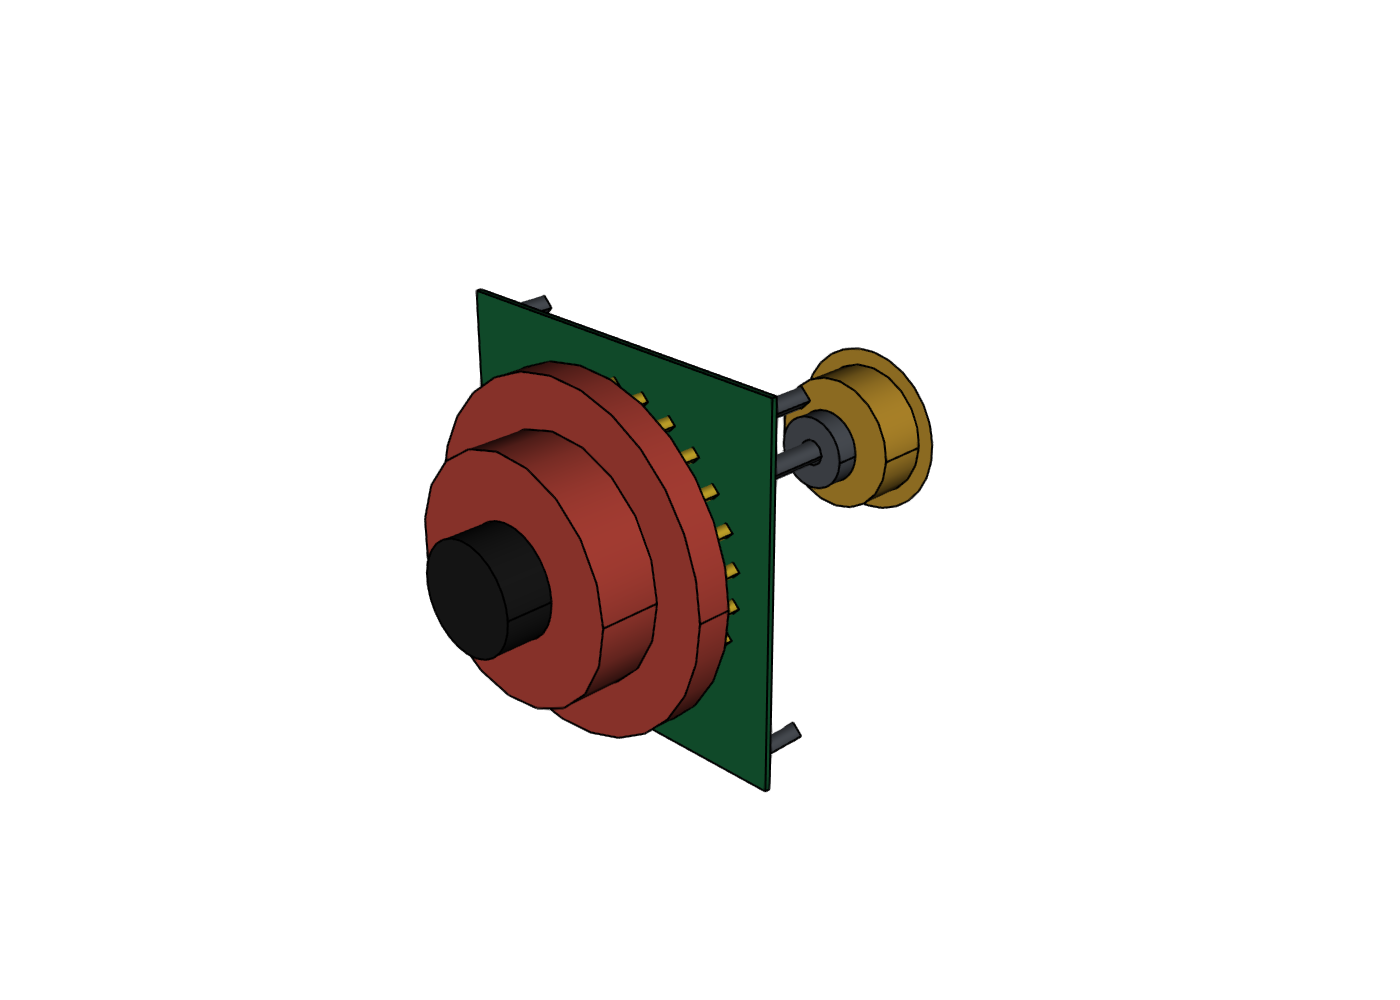
\includegraphics[width=0.48\linewidth]{../figures/generated/cad_station.png}\hfill
  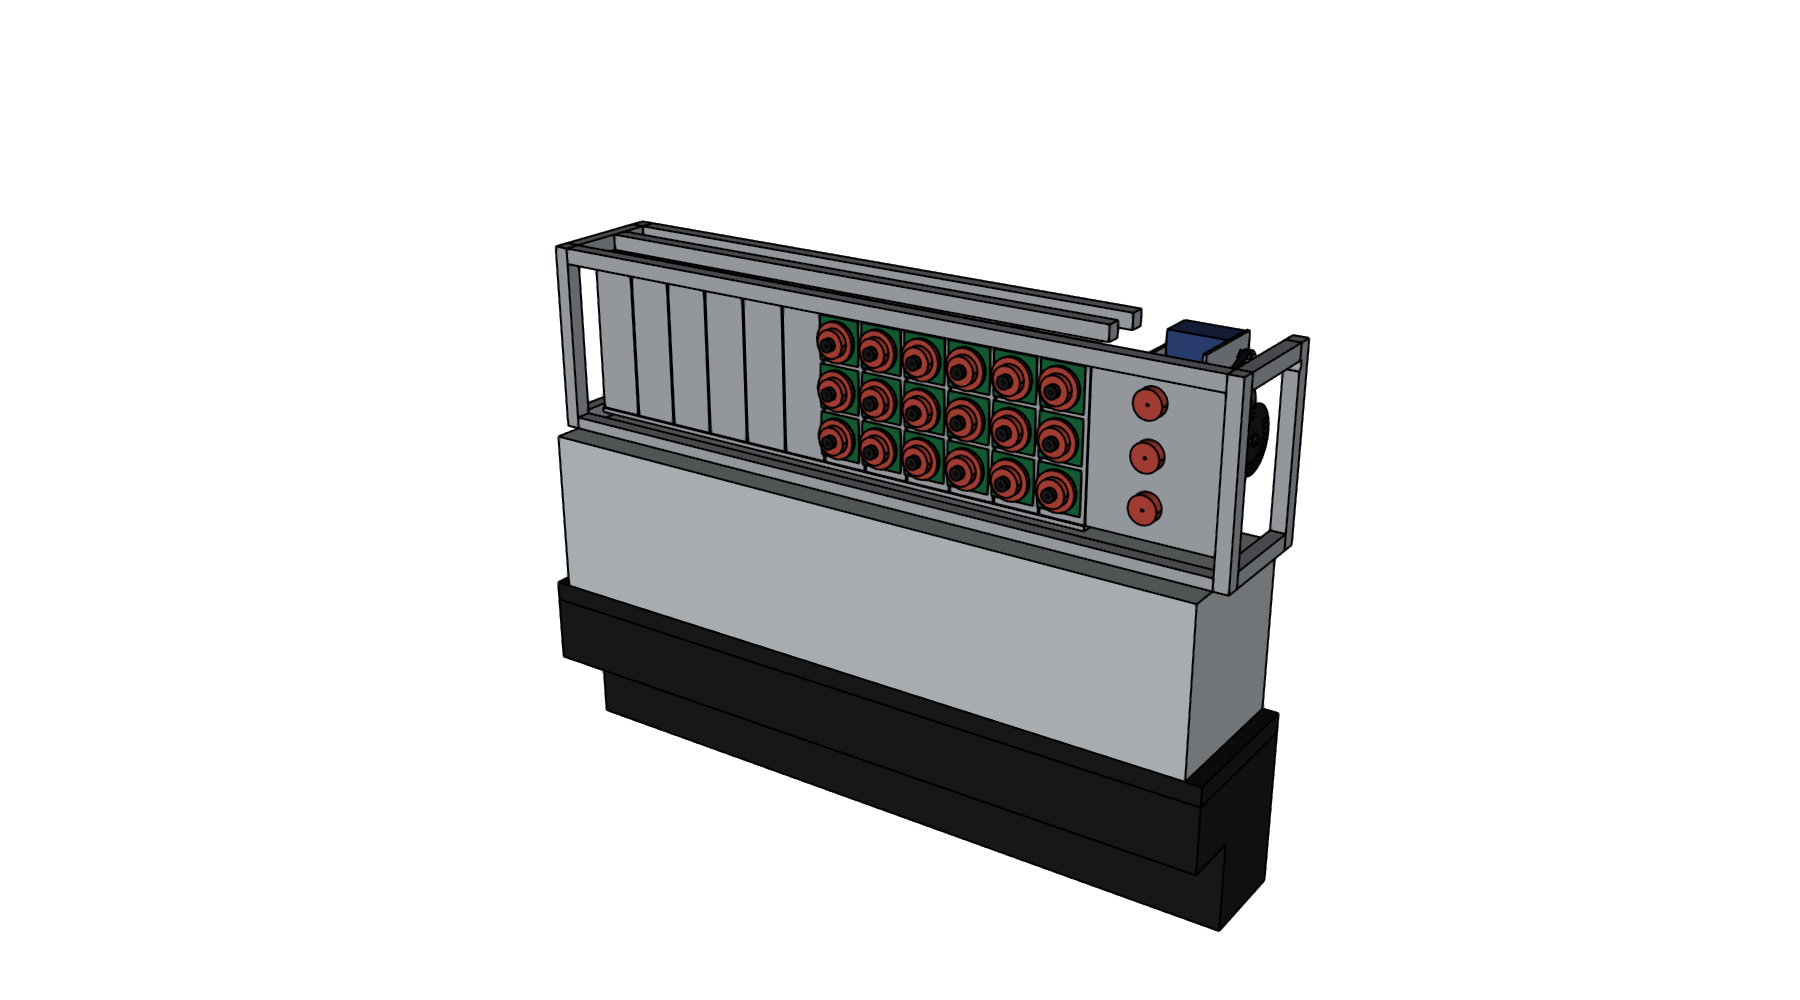
\includegraphics[width=0.48\linewidth]{../figures/generated/cad_iso.png}}{%
  \fbox{\parbox{0.9\linewidth}{\centering\footnotesize 그림 파일이 없다: \code{python hardware/gear/cad/render\_png.py}}}}
\caption{\code{render\_png.py}가 만든 그림. 왼쪽: 드럼 자리 하나(가운데 행)와 그 축의 쌓기. 오른쪽: 기계 전체(덮개를 뺀 것,
7--12번 자리에 열 모듈 여섯).}
\label{fig:gc-render}
\end{figure}

\section{정리}

\begin{itemize}
\item 기계 전체를 CadQuery 스크립트로 그린다. 숫자는 \code{params.py} 한 곳에만 있고, 숫자마다 출처(문서의 절)나
\code{(mod)}(모델링의 가정)가 붙는다. 다른 값에서 나오는 값은 계산식으로 적는다.
\item 부품은 단순한 입체의 더하기·빼기(CSG)로 만든다. 빼는 입체는 조금 넘치게 그린다. 반지름에 따라 깊어지는 V홈은 두
단면을 잇는 로프트로 판다.
\item 기계는 이름, 모양, 묶음, 역할을 가진 부품의 목록이다. 기어는 피치원으로 단순화하고, 무엇을 단순화했는지 적어 둔다.
\item \code{check.py}는 축간 거리, 패드 면, 외형, 덮개의 틈, 슬롯의 타이밍 여유를 재고, 경계 상자로 쌍을 고른 뒤 교집합
부피로 간섭을 잰다. 일부러 드럼을 1~mm 밀어 넣는 자기 시험으로 검사기 자신을 검사한다.
\item 모델이 문서의 치수 아홉 개(C1--C9)가 공간에서 닫히지 않음을 찾아냈다. 각각의 계산은 맞았지만 부품이 만나는 곳은 모델이
처음 보았다.
\item 슬롯 각도는 모터 스텝 단위로 \code{SLOT\_STEPS}에 한 번만 적고, 제어 보드의 펌웨어 모델과 시뮬레이션이 같은 파일을
읽는다.
\end{itemize}
